%%%%%%%%%%%%%%%%%%%%%%%%%%%%%%%%%%%%%%%%%%%%%%%%%%%%%%%%%%%%%%%%%%%%%%%%%%%
%%
%%  LaTeX 模板,主要针对 A4 纸的中文Paper。
%%  配合教程食用 https://mp.csdn.net/mdeditor/86517934#
%%
%%  Ver 1.0  By Tstar 
%%
%%  You can mofify it and distribute it freely :)
%%
%%%%%%%%%%%%%%%%%%%%%%%%%%%%%%%%%%%%%%%%%%%%%%%%%%%%%%%%%%%%%%%%%%%%%%%%%%%%


%%%%%%%%%%%%%%%%%%%%%%%%%%%%%%%%%%%%%%%%%%%%%%%%%%%%%%%%%%%%%%%%
%  文章模板:utf-8编码,A4 纸,10磅,文章类型为article,
%  这里设置UTF8后,下面只需要使用ctex包就能直接用中文
%%%%%%%%%%%%%%%%%%%%%%%%%%%%%%%%%%%%%%%%%%%%%%%%%%%%%%%%%%%%%%%%
\documentclass[UTF8,a4paper,10pt]{article}


%%%%%%%%%%%%%%%%%%%%%%%%%%%%%%%%%%%%%%%%%%%%%%%%%%%%%%%%%%%%%%%%
%  packages
%  这部分声明需要用到的包
%%%%%%%%%%%%%%%%%%%%%%%%%%%%%%%%%%%%%%%%%%%%%%%%%%%%%%%%%%%%%%%%
\usepackage{ctex}         % 中文支持
\usepackage{fancyhdr}
\usepackage{multicol}    % 正文单双栏混排
\usepackage{lastpage}    % 用于获得最大页数,页眉显示用
\usepackage{geometry}    % 用于设置页边距
\usepackage[subfigure,AllowH]{graphfig}    %图片相关
\usepackage{appendix}
\usepackage{graphicx}
\usepackage{amsmath}
\usepackage{booktabs}

%%%%%%%%%%%%%%%%%%%%%%%%%%%%%%%%%%%%%%%%%%%%%%%%%%%%%%%%%%%%%%%%
%定义页边距
%geometry使用手册
%http://www.ctex.org/documents/packages/layout/geometry.htm
%%%%%%%%%%%%%%%%%%%%%%%%%%%%%%%%%%%%%%%%%%%%%%%%%%%%%%%%%%%%%%%%
\geometry{left=3cm,right=3.8cm,top=2.5cm,bottom=2.5cm}
%%%%%%%%%%%%%%%%%%%%%%%%%%%%%%%%%%%%%%%%%%%%%%%%%%%%%%%%%%%%%%%%
%定义行间距为1.1倍行距
\renewcommand{\baselinestretch}{1.1}
%重新定义缩进长度  pt是字号
\parindent 22pt

%%%%%%%%%%%%%%%%%%%%%%%%%%%%%%%%%%%%%%%%%%%%%%%%%%%%%%%%%%%%%%%%
% 页眉页脚定义
% 因为首页会自动定义成plain格式 http://www.ctex.org/documents/packages/layout/fancyhdr.htm
% but我喜欢每一页都有页眉,so重定义plain型,
% 后面就全设置成plain型好了orz,其实应该改成fancy型再设置fancy的属性
%%%%%%%%%%%%%%%%%%%%%%%%%%%%%%%%%%%%%%%%%%%%%%%%%%%%%%%%%%%%%%%%
\fancypagestyle{plain}{
\fancyhf{}
\lhead{Dec., 2020}
\chead{\centering{2014-2020年长沙地区空气质量与气象因素的相关性分析}}
\rhead{Page \thepage\ of \pageref{LastPage}}
\lfoot{}
\cfoot{}
\rfoot{}}
\pagestyle{plain}

%%%%%%%%%%%%%%%%%%%%%%%%%%%%%%%%%%%%%%%%%%%%%%%%%%%%%%%%%%%%%%%%
% 标题,作者,通信地址定义
%%%%%%%%%%%%%%%%%%%%%%%%%%%%%%%%%%%%%%%%%%%%%%%%%%%%%%%%%%%%%%%%
%   texbf{...}为加粗
%   huge{...}等等调节字体的
\title{\textbf{\huge{2014-2020年长沙地区空气质量与气象因素的相关性分析}}}
\author{唐亚周 \quad 519021910804\\
电子信息与电气工程学院 \ 计算机科学与技术专业\\
}
\date{}  % 这一行用来去掉默认的日期显示


%%%%%%%%%%%%%%%%%%%%%%%%%%%%%%%%%%%%%%%%%%%%%%%%%%%%%%%%%%%%%%%%
%  文章正文
%%%%%%%%%%%%%%%%%%%%%%%%%%%%%%%%%%%%%%%%%%%%%%%%%%%%%%%%%%%%%%%%
\begin{document}
%%%%%%%%%%%%%%%%%%%%%%%%%%%%%%%%%%%%%%%%%%%%%%%%%%%%%%%%%%%%%%%%
% 此行使文献引用以上标形式显示
\newcommand{\supercite}[1]{\textsuperscript{\cite{#1}}}
%%%%%%%%%%%%%%%%%%%%%%%%%%%%%%%%%%%%%%%%%%%%%%%%%%%%%%%%%%%%%%%%
%  显示title
\maketitle

%%%%%%%%%%%%%%%%%%%%%%%%%%%%%%%%%%%%%%%%%%%%%%%%%%%%%%%%%%%%%%%%
%  中文摘要
%  调整摘要、关键词,中图分类号的页边距
%  中英文同时调整
%  因为geometry命令不能用在正文区只能用这看起来很麻烦的方法了orz
%%%%%%%%%%%%%%%%%%%%%%%%%%%%%%%%%%%%%%%%%%%%%%%%%%%%%%%%%%%%%%%%
\setlength{\oddsidemargin}{ 1cm}  % 3.17cm - 1 inch
\setlength{\evensidemargin}{\oddsidemargin}
\setlength{\textwidth}{13.50cm}
%添加标题和摘要的距离
%vspace{...}是竖直距离
%hspace{...}是水平距离
\vspace{-0.2cm}
%center是居中用的
\begin{center}
%在这里写中文摘要
%heiti表示....黑体,kaishu是楷书,还有songti宋体,lishu隶书,fangsong仿宋
\parbox{\textwidth}{
{\heiti 摘~~~要}\quad {\kaishu 一直以来,空气质量问题都是我国城市化发展过程中亟待解决的难题。长沙市作为一座快速发展的新一线城市,空气质量问题自然十分关键。本文以天为单位,通过分析以PM2.5为代表的空气质量指数和当天的天气状况、气温、风速等指标的关系,得出一系列结论。}\\\\
{\heiti 关键词} \quad {\kaishu 空气质量,长沙,天气,量化分析}}
\end{center}
\vspace{0.5cm}

%%%%%%%%%%%%%%%%%%%%%%%%%%%%%%%%%%%%%%%%%%%%%%%%%%%%%%%%%%%%%%%%
%  目录页-------------------------
%%%%%%%%%%%%%%%%%%%%%%%%%%%%%%%%%%%%%%%%%%%%%%%%%%%%%%%%%%%%%%%%
\newpage
\tableofcontents
\newpage

%%%%%%%%%%%%%%%%%%%%%%%%%%%%%%%%%%%%%%%%%%%%%%%%%%%%%%%%%%%%%%%%
%  正文由此开始-------------------------
%%%%%%%%%%%%%%%%%%%%%%%%%%%%%%%%%%%%%%%%%%%%%%%%%%%%%%%%%%%%%%%%
%%%%%%%%%%%%%%%%%%%%%%%%%%%%%%%%%%%%%%%%%%%%%%%%%%%%%%%%%%%%%%%%
%  恢复正文页边距
%%%%%%%%%%%%%%%%%%%%%%%%%%%%%%%%%%%%%%%%%%%%%%%%%%%%%%%%%%%%%%%%
\setlength{\oddsidemargin}{1cm}  % 3.17cm - 1 inch
\setlength{\evensidemargin}{\oddsidemargin}
\setlength{\textwidth}{17.00cm}

\section{研究背景}
%\indent 为首行缩进
%引用文献
\indent 近期召开的十九届五中全会审议通过的《中共中央关于制定国民经济和社会发展第十四个五年规划和二〇三五年远景目标的建议》(以下简称《建议》),从多个方面对生态文明建设和生态环境保护作出重要部署、提出明确要求,为做好“十四五”生态环境保护工作指明了前进方向、提供了根本遵循。2021年是我国现代化建设进程中具有特殊重要性的一年,也是“十四五”时期的开局之年,要立足新发展阶段,坚持新发展理念,构建新发展格局,把生态文明建设和生态环境保护作为推动高质量发展的题中应有之义,进一步凸显其重要地位和关键作用,抓紧谋划“十四五”生态环境保护工作,坚持稳中求进工作总基调,对标对表2035年远景目标,牢固树立落实绿水青山就是金山银山的理念,促进经济社会发展全面绿色转型,加快推动绿色低碳发展,持续改善环境质量,提升生态系统质量和稳定性,全面提高资源利用效率,更加注重系统观念在生态环境保护工作中的科学运用和实践深化,突出精准治污、科学治污、依法治污,更好发挥生态环境保护对高质量发展、构建新发展格局的支撑服务保障作用,为开启全面建设社会主义现代化国家新征程、向第二个百年奋斗目标进军奠定坚实基础。\supercite{ref1}\\
\indent 在这样的大背景下,借这次概率统计课程大作业的机会,本人决定对家乡长沙的空气质量进行一次研究。\\

\section{前期准备}

\subsection{文献调研}
\indent 经过查阅资料\supercite{ref2}得知,空气质量的主要影响因素有局地污染和西北地区沙尘传输造成的自然降尘、气象要素(降水量、风速、逆温等)、地形的空间差异和人类活动等多个方面。考虑到长沙市的地理特征、产业结构以及数据收集的难易程度,我选择对气象因素和空气质量的关系进行研究。 

\subsection{数据搜集及处理}
\indent 本人在网络\supercite{ref3}上搜集到2014年到2020年长沙市的空气质量指数,再利用python爬虫在网络\supercite{ref4}上获取2014年到2020年长沙市的气象要素数据。然后去除数据集中的无效数据,得到2531个有效数据。

\section{数据分析}
\subsection{空气质量指数与温度的关系}
\indent 收集到的数据中,有当日最高温度和最低温度两个数据,将这两个数据求平均值处理,得到的值作为一天的温度。以年份为单位,将温度及PM2.5和日期的关系进行可视化,如图\ref{Fig.main1}所示

\begin{figure}[H] %H为当前位置,!htb为忽略美学标准,htbp为浮动图形
\centering %图片居中
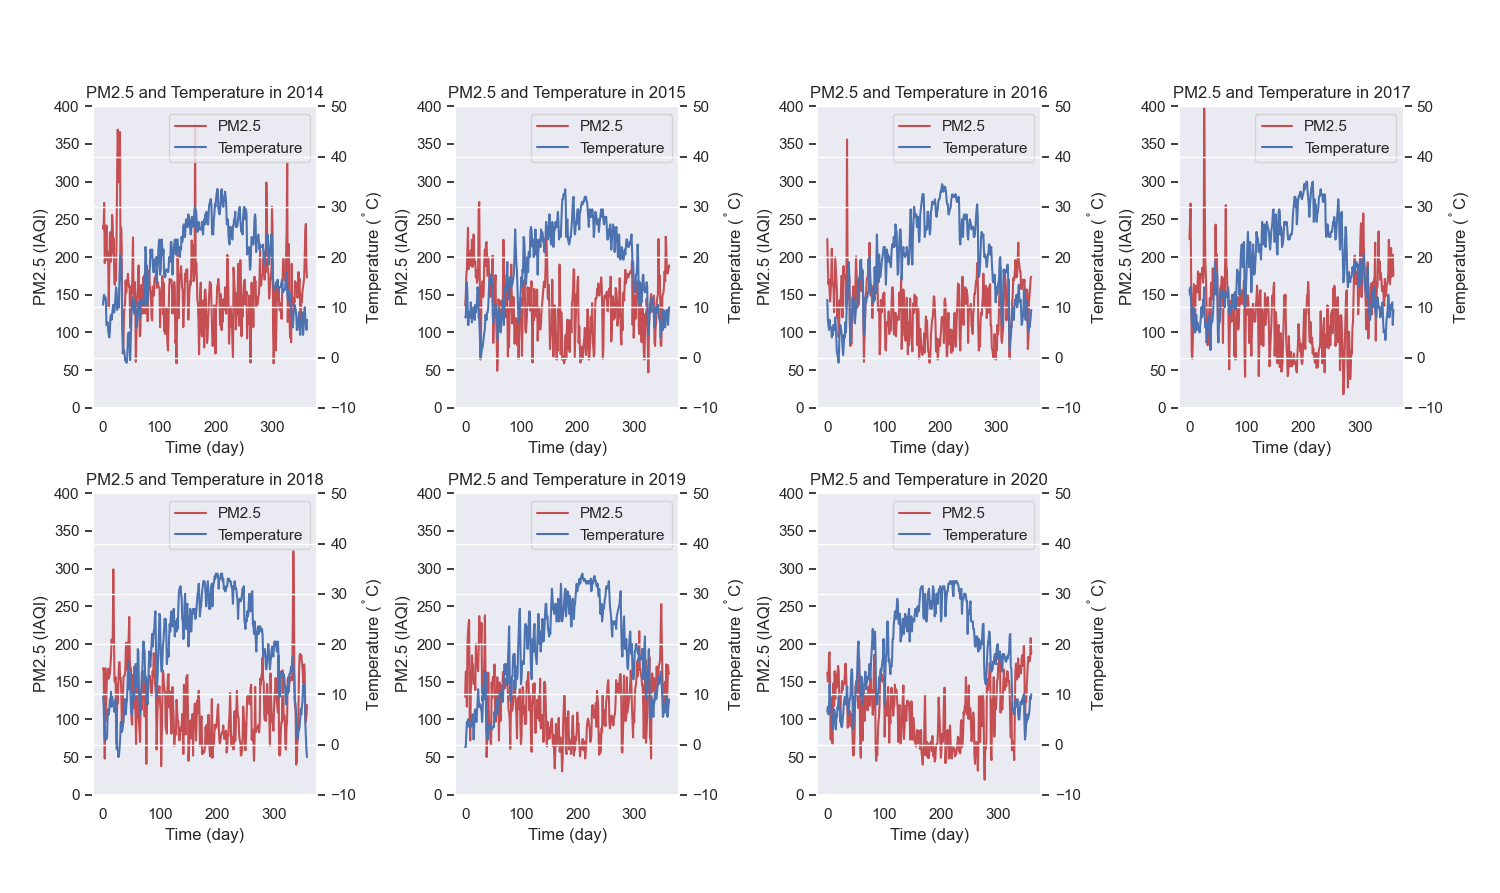
\includegraphics[width=0.7\textwidth]{fig//pm25-temp-alltime.png} %插入图片,[]中设置图片大小,{}中是图片文件名
\caption{2014-2020年长沙地区各年PM2.5指数及气温与日期的关系图} %最终文档中希望显示的图片标题
\label{Fig.main1} %用于文内引用的标签
\end{figure}

\indent 可以看出,总体上PM2.5指数与气温呈负相关。然后对于PM2.5指数和气温绘制二维直方图,如图\ref{Fig.main2}所示,并使用Python内置函数计算相关系数。

\begin{figure}[H] %H为当前位置,!htb为忽略美学标准,htbp为浮动图形
\centering %图片居中
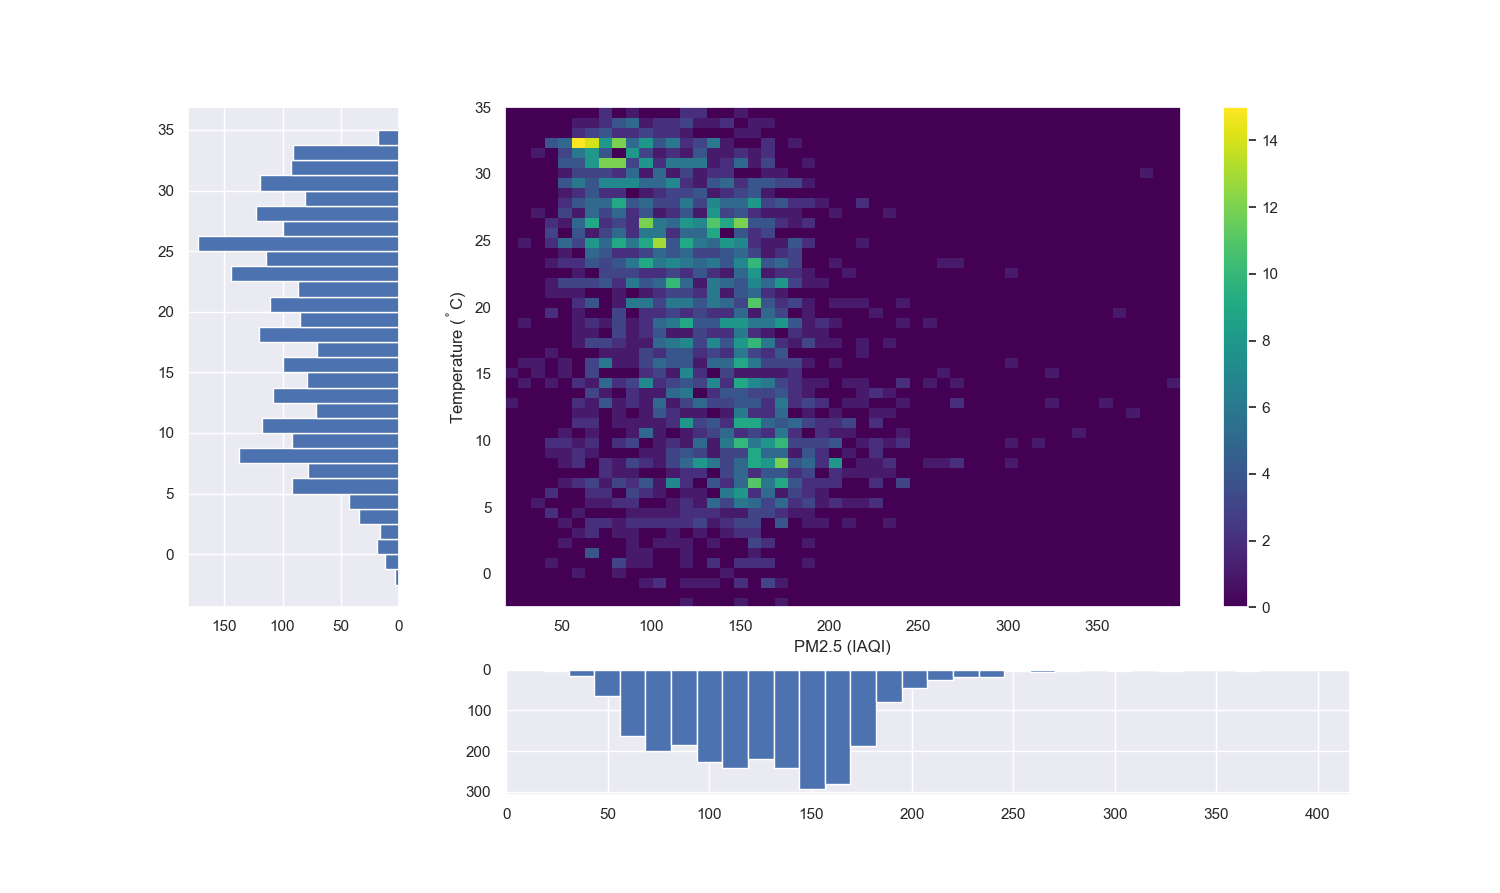
\includegraphics[width=0.7\textwidth]{fig//pm25-temp.png} %插入图片,[]中设置图片大小,{}中是图片文件名
\caption{2014-2020年长沙地区PM2.5指数与气温的分布图} %最终文档中希望显示的图片标题
\label{Fig.main2} %用于文内引用的标签
\end{figure}

\begin{equation}
\rho_{XY} =  \frac{\operatorname{cov}(X, Y)}{\sqrt{\operatorname{D}(X) \cdot \operatorname{D}(Y)}} = -0.35
\end{equation}
\indent 由此看出,PM2.5指数与温度呈一定的负相关,但相关性并不明显。

\subsection{空气质量指数与天气状况的关系}

\indent 通过遍历数据,我们得到了7年来长沙地区出现过的所有天气情况,并按照降雨量/降雪量的大小将其分级,如表\ref{table1}所示。

\begin{table}[]
    \caption{天气状况及人为分级}
    \vspace{20pt}
    \centering
    \begin{tabular}{ccc}
        \toprule  %添加表格头部粗线
        天气情况& 级别& 分级依据\\
        \midrule  %添加表格中横线
        晴& 1& 一般为干燥\\
        多云& 1& 一般为干燥天气\\
        阴& 2& 一般湿度比较大,但没有降水\\
        小雨& 3& 一般降水量较少\\
        小到中雨& 3& 一般降水量较少\\
        阵雨& 3& 一般降水量较少\\
        雷阵雨& 3& 一般降水量较少\\
        雨& 3& 一般降水量较少\\
        中雨& 4& 一般降水量较大\\
        中到大雨& 4& 一般降水量较大\\
        大雨& 4& 一般降水量较大\\
        大到暴雨& 4& 一般降水量较大\\
        暴雨& 4& 一般降水量较大\\
        冻雨& 3& 一般降水量较少\\
        雨夹雪& 3& 一般降水量较少\\
        小雪& 3& 一般降水量较少\\
        小雪-中雪& 3& 一般降水量较少\\
        中雪& 4& 一般降水量较大\\
        中到大雪& 4& 一般降水量较大\\
        大雪& 4& 一般降水量较大\\
        \bottomrule %添加表格底部粗线       
    \end{tabular}
    \label{table1}
\end{table}

\indent 将数据中每天的两个天气信息及其对应的级别均记录下来,也就是说一个空气质量的信息对应着两个天气状况信息。得到1级天气2568次、2级天气544次、3级天气1592次、四级天气358次。
\newpage 对四种天气下的PM2.5指数做统计,得到直方图如图\ref{Fig.main3}所示。

\begin{figure}[H] %H为当前位置,!htb为忽略美学标准,htbp为浮动图形
\centering %图片居中
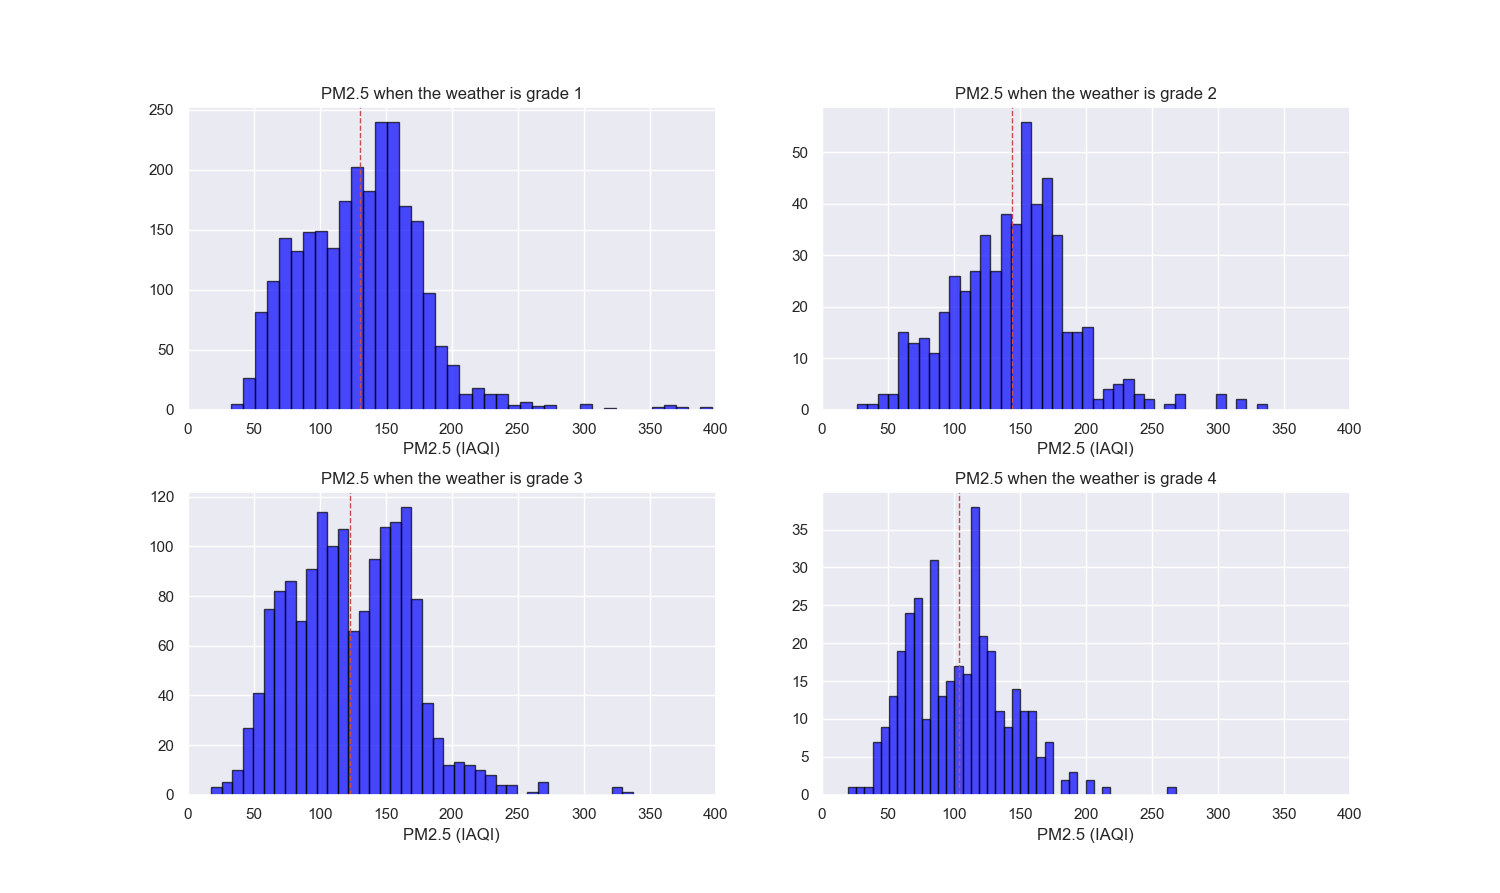
\includegraphics[width=0.7\textwidth]{fig//pm25-weather.png} %插入图片,[]中设置图片大小,{}中是图片文件名
\caption{2014-2020年间长沙地区4钟天气情况下的PM2.5指数分布直方图} %最终文档中希望显示的图片标题
\label{Fig.main3} %用于文内引用的标签
\end{figure}

\indent 由$E(X)=\sum_{i=1}^{n} x_{i} p_{i}$和$D(X)=\sum_{i=1}^{n}\left[x_{i}-E(X)\right]^{2} p_{i}$可计算出四种天气下PM2.5指数的期望和方差,如表\ref{table2}所示。

\begin{table}[]
    \caption{各级别天气下PM2.5指数的样本期望和方差}
    \vspace{20pt}
    \centering
    \begin{tabular}{ccc}
        \toprule  %添加表格头部粗线
        天气级别& 期望& 方差\\
        \midrule  %添加表格中横线
        级别1& 130.87& 2032.00\\
        级别2& 143.81& 2051.42\\
        级别3& 123.16& 1993.46\\
        级别4& 104.01& 1392.35\\
        \bottomrule %添加表格底部粗线       
    \end{tabular}
    \label{table2}
\end{table}

\newpage \indent 可以看到,总体上来说,当天气的级别越高,也就是降水量越大、空气越湿润时,PM2.5指数总体上越小。另外,我们可以按照国家标准\supercite{ref5}里所规定的”中度污染“以上的标准,也就是PM2.5的IAQI值大于等于151的情况下,对四种级别的天气进行统计,如图\ref{Fig.main4}和表\ref{table3}所示。可以看到,总体上来说,当天气的级别越高,出现”中度污染“及以上的比例要减小。
\indent 但是在级别2的天气(阴天)时,PM2.5指数的期望要比级别1(晴天和多云)要大,出现”中度污染“及以上的次数比例也要高于级别1。综上所述,PM2.5指数在不同天气下从高到低排序应该是$2>1>3>4$。


\begin{figure}[H] %H为当前位置,!htb为忽略美学标准,htbp为浮动图形
\centering %图片居中
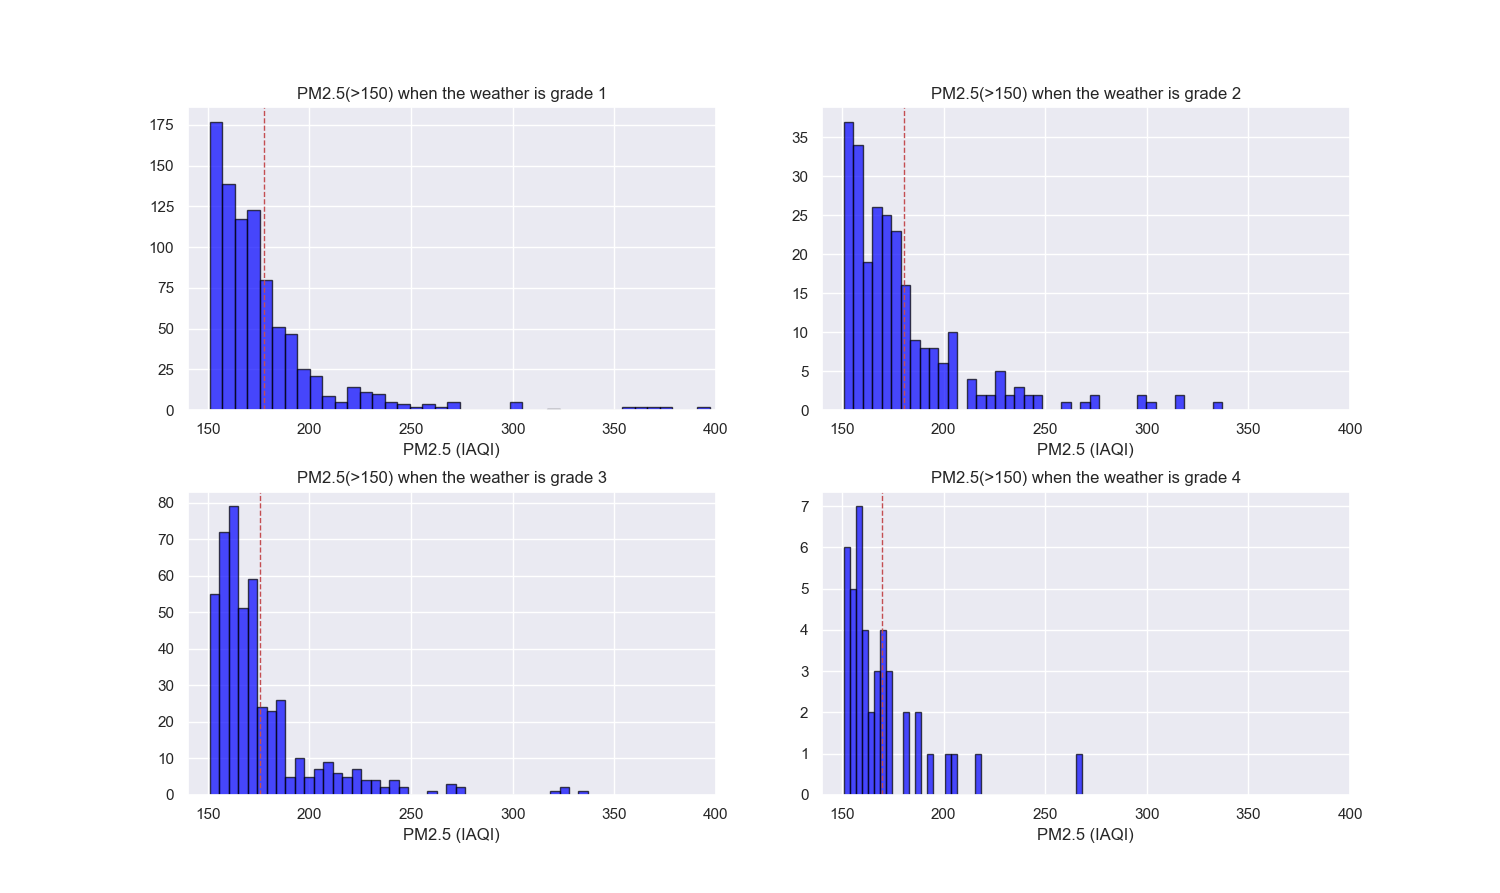
\includegraphics[width=0.7\textwidth]{fig//pm25-weather-serious.png} %插入图片,[]中设置图片大小,{}中是图片文件名
\caption{2014-2020年间长沙地区4钟天气情况下的PM2.5指数分布直方图(中度污染及以上)} %最终文档中希望显示的图片标题
\label{Fig.main4} %用于文内引用的标签
\end{figure}

\begin{table}[]
    \caption{各级别天气下中度污染及以上天数的样本期望和数量}
    \vspace{20pt}
    \centering
    \begin{tabular}{cccc}
        \toprule  %添加表格头部粗线
        天气级别& 期望& 出现次数& 占总数比例\\
        \midrule  %添加表格中横线
        级别1& 177.79& 867& $33.67\%$ \\
        级别2& 180.49& 253& $46.51\%$ \\
        级别3& 175.75& 469& $29.46\%$ \\
        级别4& 169.62& 43& $12.01\%$ \\
        \bottomrule %添加表格底部粗线       
    \end{tabular}
    \label{table3}
\end{table}

\subsection{空气质量指数与风速的关系}

\indent 考虑到风力等级与风速并非线性关系,直接将一天中的两个风力等级数据取平均值作为一天的风力等级并不合理。故同样选择将数据中每天的两个风力等级均记录下来,也就是说一个空气质量的信息对应着两个风力等级信息。得到1级风779次,2级风779次,3级风3110次,4级风363次,5级风28次,6级风3次。然后按照3.2节中相同的处理方式,如表\ref{table4}和图\ref{Fig.main5}所示。

\begin{figure}[H] %H为当前位置,!htb为忽略美学标准,htbp为浮动图形
\centering %图片居中
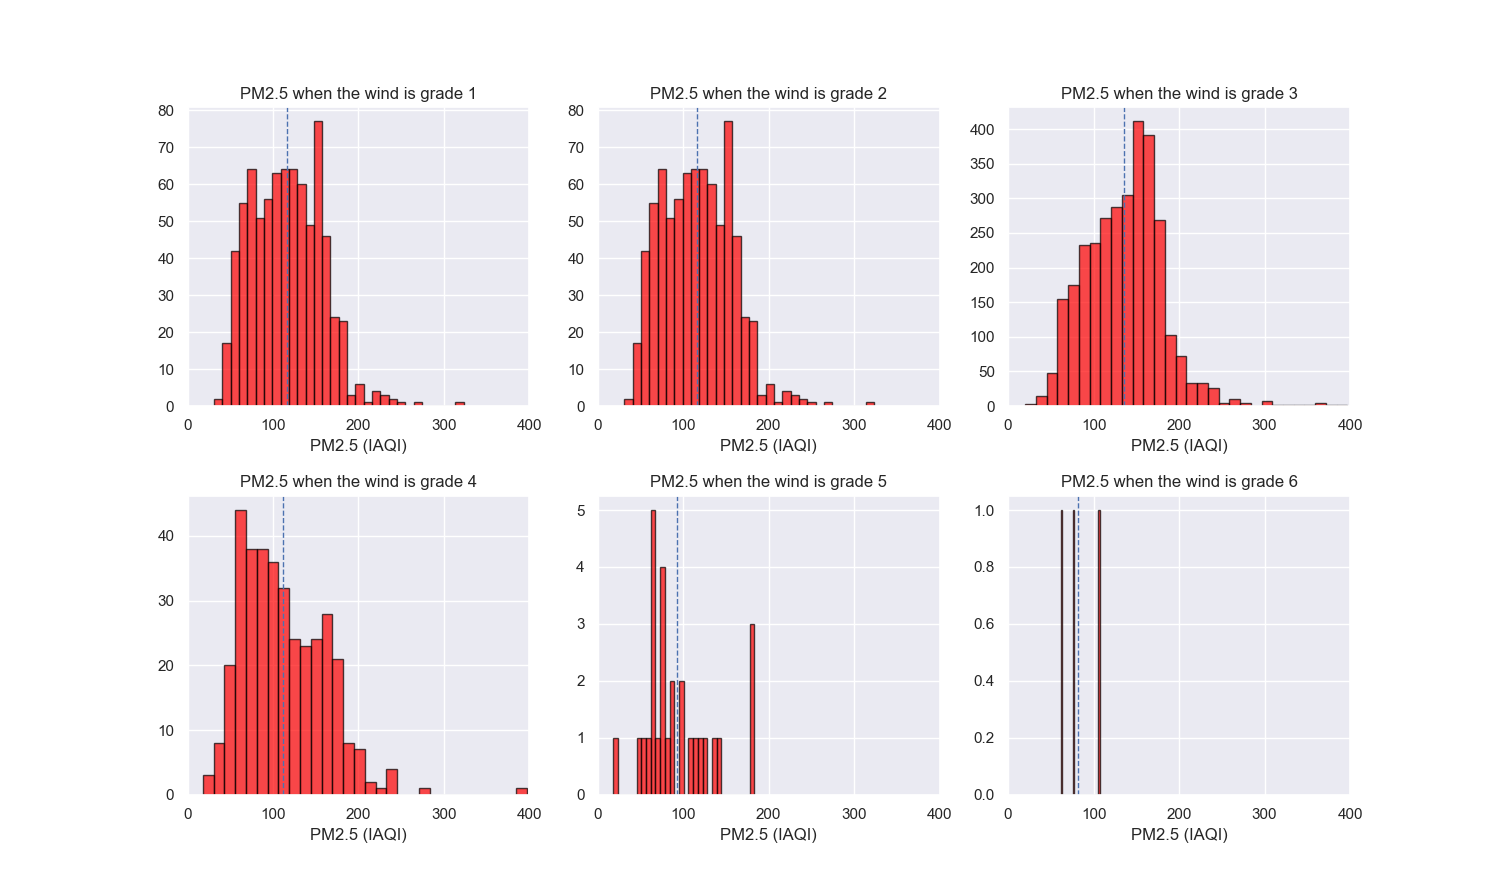
\includegraphics[width=0.7\textwidth]{fig//pm25-wind.png} %插入图片,[]中设置图片大小,{}中是图片文件名
\caption{2014-2020年间长沙地区不同风力等级下的PM2.5指数分布直方图} %最终文档中希望显示的图片标题
\label{Fig.main5} %用于文内引用的标签
\end{figure}

\begin{table}[]
    \caption{各级别风力下PM2.5指数的样本期望以及“中度污染”及以上天数比例}
    \vspace{20pt}
    \centering
    \begin{tabular}{cccc}
        \toprule  %添加表格头部粗线
        风力等级& 期望& “中度污染”及以上空气出现次数& “中度污染”及以上天数占总数比例\\
        \midrule  %添加表格中横线
        级别1& 115.96& 168& $21.57\%$\\
        级别2& 115.96& 168& $21.57\%$\\
        级别3& 136.13& 1210& $38.91\%$\\
        级别4& 112.13& 83& $22.87\%$\\
        级别5& 93.04& 3& $10.71\%$\\
        级别6& 81.67& 0& $0\%$\\
        \bottomrule %添加表格底部粗线       
    \end{tabular}
    \label{table4}
\end{table}



%\begin{Figure}[H]{aaa}[qwad]
%%pic和tex文件保存在同一路径下
%\graphfile[30]{1.png}[picture]
%%相对路径(推荐),可以在tex所在路径建立一个fig 文件夹放图片
%%\graphfile[60]{fig//1.png}[picture]
%%绝对路径,从电脑任意位置寻找图片
%%\graphfile[30]{C://Users//TstarYSY//Desktop//fig//1.png}[picture]
%\end{Figure}
%% \noindent 取消首行缩进
%\noindent 南无阿弥陀佛南无阿弥陀佛南无阿弥陀佛南无阿弥陀佛南无阿弥陀佛\par
%南无阿弥陀佛南无阿弥陀佛南无阿弥陀佛南无阿弥陀佛南无阿弥陀佛南无阿弥陀佛南无阿弥陀佛南无阿弥陀佛南无阿弥陀佛南无阿弥陀佛南无阿弥陀佛南无阿弥陀佛南无阿弥陀佛南无阿弥陀佛
%\par
%\begin{Figure}[H]{asdf}[111]
%\graphfile[34]{1.png}[picture1]
%\graphfile[36]{1.png}[picture2]
%\par
%\end{Figure}

\section{结论与展望}
南无阿弥陀佛南无阿弥陀佛南无阿弥陀佛南无阿弥陀佛南无阿弥陀佛南无阿弥陀佛南无阿弥陀佛南无阿弥陀佛南无阿弥陀佛南无阿弥陀佛南无阿弥陀佛南无阿弥陀佛
\par

\noindent 南无阿弥陀佛南无阿弥陀佛南无阿弥陀佛南无阿弥陀佛南无阿弥陀佛南无阿弥陀佛南无阿弥陀佛南无阿弥陀佛南无阿弥陀佛南无阿弥陀佛南无阿弥陀佛南无阿弥陀佛
\section{公式}
南无阿弥陀佛南无阿弥陀佛南无阿弥陀佛南无阿弥陀佛南无阿弥陀佛南无阿弥陀佛南无阿弥陀佛南无阿弥陀佛南无阿弥陀佛南无阿弥陀佛南无阿弥陀佛南无阿弥陀佛南无阿弥陀佛南无阿弥陀佛南无阿弥陀佛南无阿弥陀佛南无阿弥陀佛南无阿弥陀佛南无阿弥陀佛南无阿弥陀佛南无阿弥陀佛南无阿弥陀佛南无阿弥陀佛南无阿弥陀佛
\noindent

\par\noindent
南无阿弥陀佛南无阿弥陀佛南无阿弥陀佛南无阿弥陀佛南无阿弥陀佛南无阿弥陀佛南无阿弥陀佛南无阿弥陀佛南无阿弥陀佛南无阿弥陀佛南无阿弥陀佛南无阿弥陀佛
\section{结束}


\begin{itemize}
    \item 身是菩提树,心如明镜台
    \item 时时勤拂拭,勿使惹尘埃.
    \item 菩提本无树,明镜亦非台
    \item 本来无一物,何处惹尘埃.
\end{itemize}

\vspace{3ex}
\begin{table}[h]
    \centering
    %{|l|c|c|}指明有3列而且对其方式是左中中,|表示要加竖线
    %\hline表示添加横线
    \begin{tabular}{|l|c|c|}\hline
        %&表示一个单元格内容结束
        %multicolumn{n}{...}{...}表示合并n个单元格,指明对齐方式和内容
        Setting&\multicolumn{2}{c|}{A4 size paper}\\\hline
        &mm&inches\\
        Top&25&1.0\\
        Bottom&25&1.0\\
        Left&20&0.8\\
        Right&20&0.8\\
        Column Width&82&3.2\\
        Column Spacing&6&0.25\\\hline
    \end{tabular}
    \caption{a table}
    \label{tab:table1}
\end{table}
\vspace{3ex}

\begin{figure}[h]
\begin{minipage}[h]{0.48\linewidth}
\[\alpha  \ge \delta {\rm{ + }}\overline {\eta  * \beta } \]
\end{minipage}
\begin{minipage}[h]{0.48\linewidth}
\[\left[ {\begin{array}{*{20}{c}}
{{a_1}}&{{a_2}}&\alpha &\beta \\
\chi &\varphi &\gamma &\eta \\
\theta &{{\zeta _3}}&\xi &\omega
\end{array}} \right]\]
\end{minipage}
\vspace{3ex}
\caption{aaa}
\end {figure}

%%%%%%%%%%%%%%%%%%%%%%%%%%%%%%%%%%%%%%%%%%%%%%%%%%%%%%%%%%%%%%%%
%  参考文献
%%%%%%%%%%%%%%%%%%%%%%%%%%%%%%%%%%%%%%%%%%%%%%%%%%%%%%%%%%%%%%%%
\small
\begin{thebibliography}{99}
    \setlength{\parskip}{0pt}  %段落之间的竖直距离
    \bibitem{ref1} 中华人民共和国生态环境部.生态环境部举行党的十九届五中全会精神辅导报告会[EB/OL].https://www.mee.gov.cn/xxgk2018/xxgk/xxgk15/202012/t20201212812690.html,2020-12-12.
    % 这里应该是t20201212_812690.html
    \bibitem{ref2} 李小飞,张明军,王圣杰,赵爱芳,马潜.中国空气污染指数变化特征及影响因素分析[J].环境科学,2012,33(06):1936-1943.
    \bibitem{ref3} The World Air Quality Project.Air Quality Historical Data Platform[DB/OL].https://aqicn.org/data-platform/register/,2020-12-26.
    \bibitem{ref4} 天气网.历史天气查询[DB/OL].http://lishi.tianqi.com/,2020-12-26.
    \bibitem{ref5} HJ 633—2012,环境空气质量指数(AQI)技术规定(试行)[S].中国:中华人民共和国生态环境部,2012.

\end{thebibliography}

\begin{appendices}
    \section{Python爬虫代码}
    some text in Appendix A
    \section{Python数据分析代码}
    some text in Appendix B
 \end{appendices}

%%%%%%%%%%%%%%%%%%%%%%%%%%%%%%%%%%%%%%%%%%%%%%%%%%%%%%%%%%%%%%%%
%  文章结束
%%%%%%%%%%%%%%%%%%%%%%%%%%%%%%%%%%%%%%%%%%%%%%%%%%%%%%%%%%%%%%%%
\clearpage
\end{document}